%!TEX root = ../icip_jseo.tex
% -*- root: ../icip_jseo.tex -*-


\section{Experiments}

% 앞에서 제안한 특징점 Filtering 알고리즘을 이용하여 학습을 수행하였을 때 인식 성능의 개선을 측정하였다. 

% 실험 영상은, 서울시 가이드 지도 팜플릿 영상 16장을 선택하여 사용되었다. 이러한 영상을 rotation($0.5\sim2.0$배, 0.1배 간격), scale($0\degree\sim360\degree$, $10\degree$ 간격), blur(Gaussian blur, $r=0,3,5,7$pixels) 등의 변형(deformed)한 영상 32,256장 중 random sampling하여 train images 16,114장, test images 16,142장을 선택하였다.
% 먼저 train images에서 특징점들을 검출(detect)하고, detected keypoint 들을 이용하여 앞의 정의된 Score function($gf(p_i)$)을 계산하였다. 

In this chapter, we present several experiments that demonstrate the effectiveness of the proposed method. As for the experimental images, 16 images of Seoul Guide Map Pamphlet was selected. These images were deformed by way of rotating($0.5\sim2.0$-folds, at the interval of 0.1-fold) scaling (($0\degree\sim360\degree$, at the interval of $10\degree$ intervals) and blurring (Gaussian blur, $r = 0,3,5,7$ pixels). As a result, 32,256 images were obtained. Of them, 16,114 training images and 16,142 test images were selected at random. With training images, we detected keypoints and calculated the score function($gf(p_i)$). Then, we stored filtered keypoints and calculated nearest neighbor with test images.

At first, to prove the proposed algorithm can enhance recognition performance, we conducted a comparison experiment(see, Fig. \ref{fig:comparison_agast_freak}). Keypoints are detected with AGAST\cite{mair_adaptive_2010} detector and described with FREAK\cite{alahi_freak:_2012} descriptor. The figure shows comparison among top 50 keypoints based on the proposed score function(\textit{Proposed}), 50 keypoints filtered randomly(\textit{Random}), top 50 keypoints based on the corner response function(\textit{C.R.F.}), and non-filtered $3,000$ keypoints set(\textit{Full}). The figure shows that the proposed approach generates the most robust matching performance.

\begin{figure}[ht!]
\centering
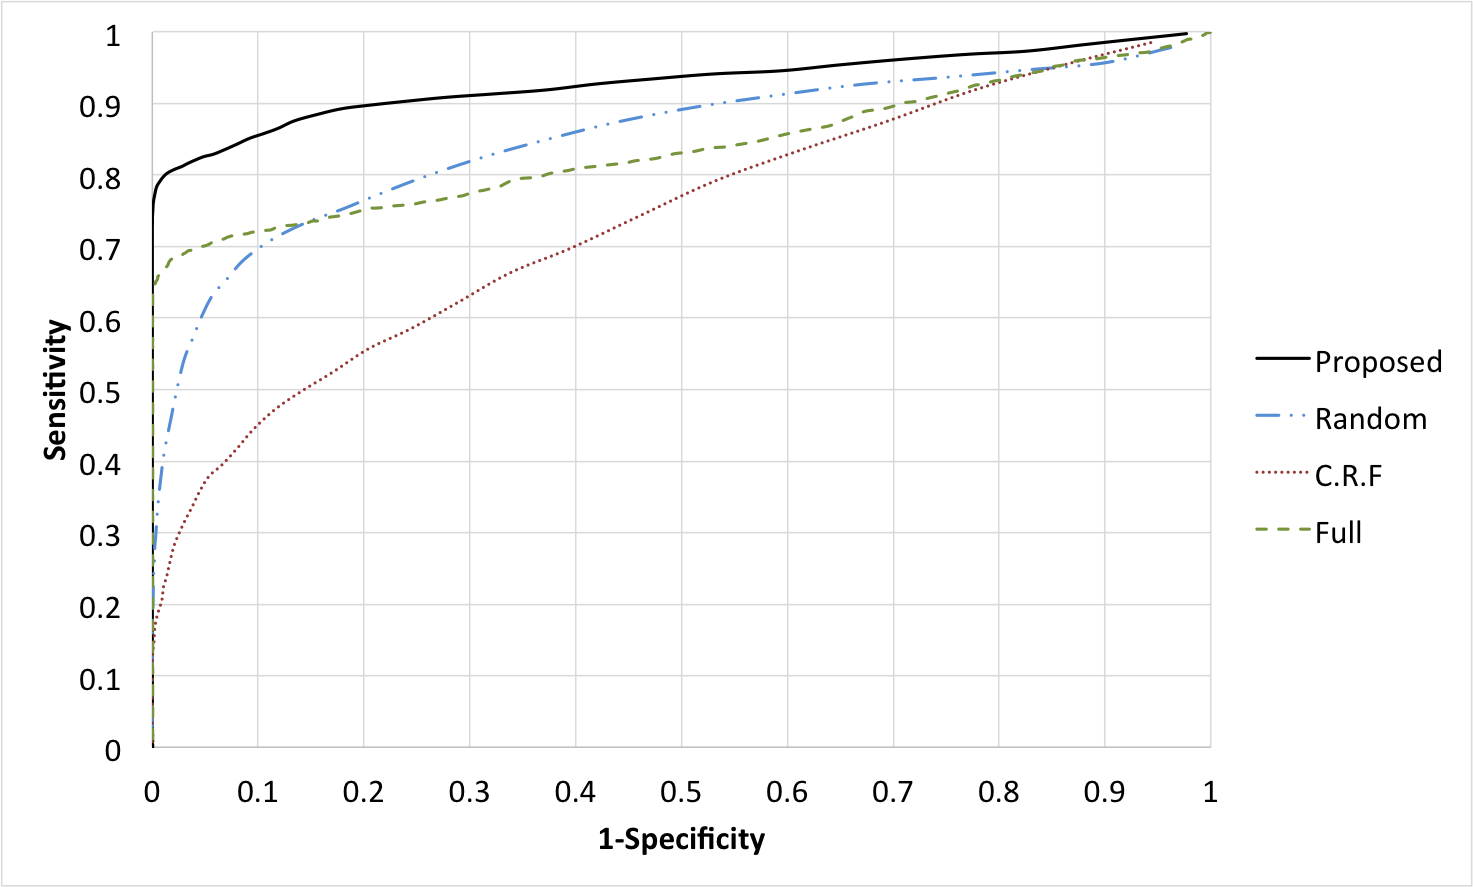
\includegraphics[width=1.0\columnwidth]{4_experiments/comparison_agast_freak}
\caption{ROC curve comparison between proposed filtering function and other methods}
\label{fig:comparison_agast_freak}
\end{figure}

At second, to prove the proposed approach works among several algorithm suits, we performed the comparison tests with changing detection and description algorithms(see, Fig. \ref{algorithm_comparison}). These figures show the proposed method generates robust matching performance even though the algorithm is changed.

\begin{figure}[hb!]
  \centering     %%% not \center
    \subfigure[AGAST detector and BRISK descriptor]{\label{fig:agast_brisk}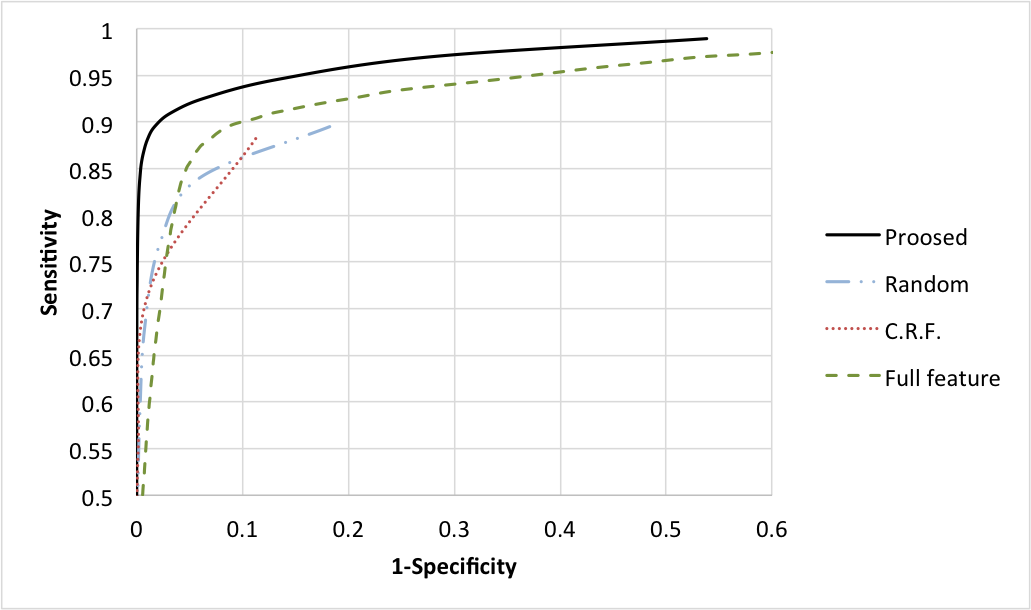
\includegraphics[width=1.0\columnwidth]{4_experiments/agast_brisk}}
    \\
    \subfigure[SURF detector and FREAK descriptor]{\label{fig:surf_freak}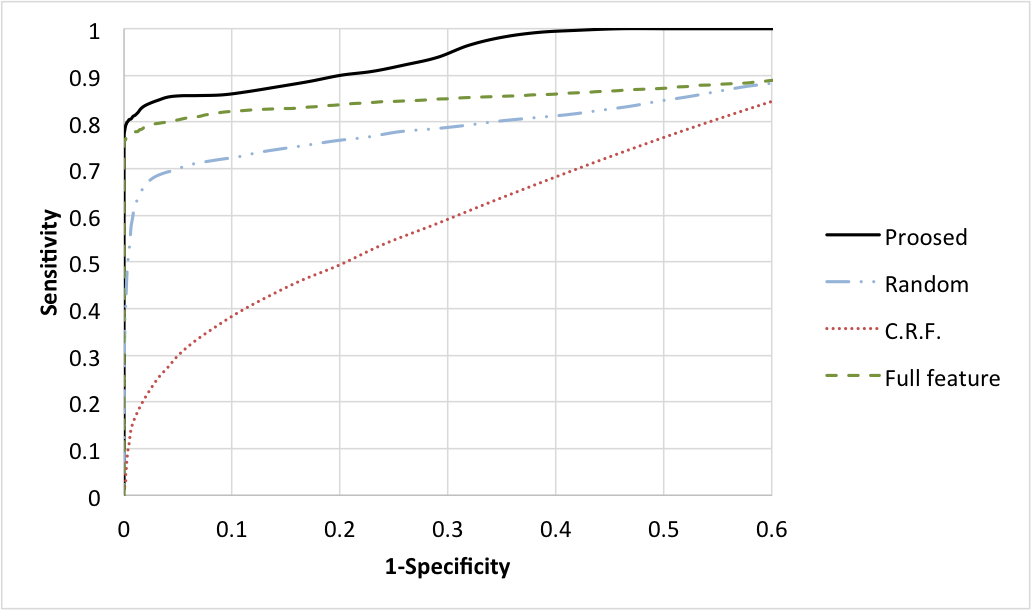
\includegraphics[width=1.0\columnwidth]{4_experiments/surf_freak}}
  \caption{ROC curve comparison between different algorithm sutirs}
    \label{fig:algorithm_comparison}
\end{figure}

%특징점 데이터베이스는 Score function을 고려하지 않은 전체 특징점 집합($K_{all}, n(K_{all}) = 3000$)과, Score function에서 상위 50개, 100개, 300개, 500개 특징점들만 filtering 하여 구성한 특징점 집합($K_{50}, K_{100}, K_{300}, K_{500}$)으로 구성되었다. 

The last experiment is performed to calculate the optimal number of keypoints. The experiment is performed among non-filtered 3,000 keypoints set($K_{all}$), top 500, 300, 100, 50 keypoints subsets($K_{500, 300, 100, 50}$). As shown Fig. \ref{fig:markerless_roc}, the result showed slight degradation of recognition rate whereas $K_{100}$ and $K_{50}$ showed the improvement of performance.  

%%%%%분석 결과가 더 들어가면 좋겠다%%%%%


\begin{figure}[ht!]
\centering
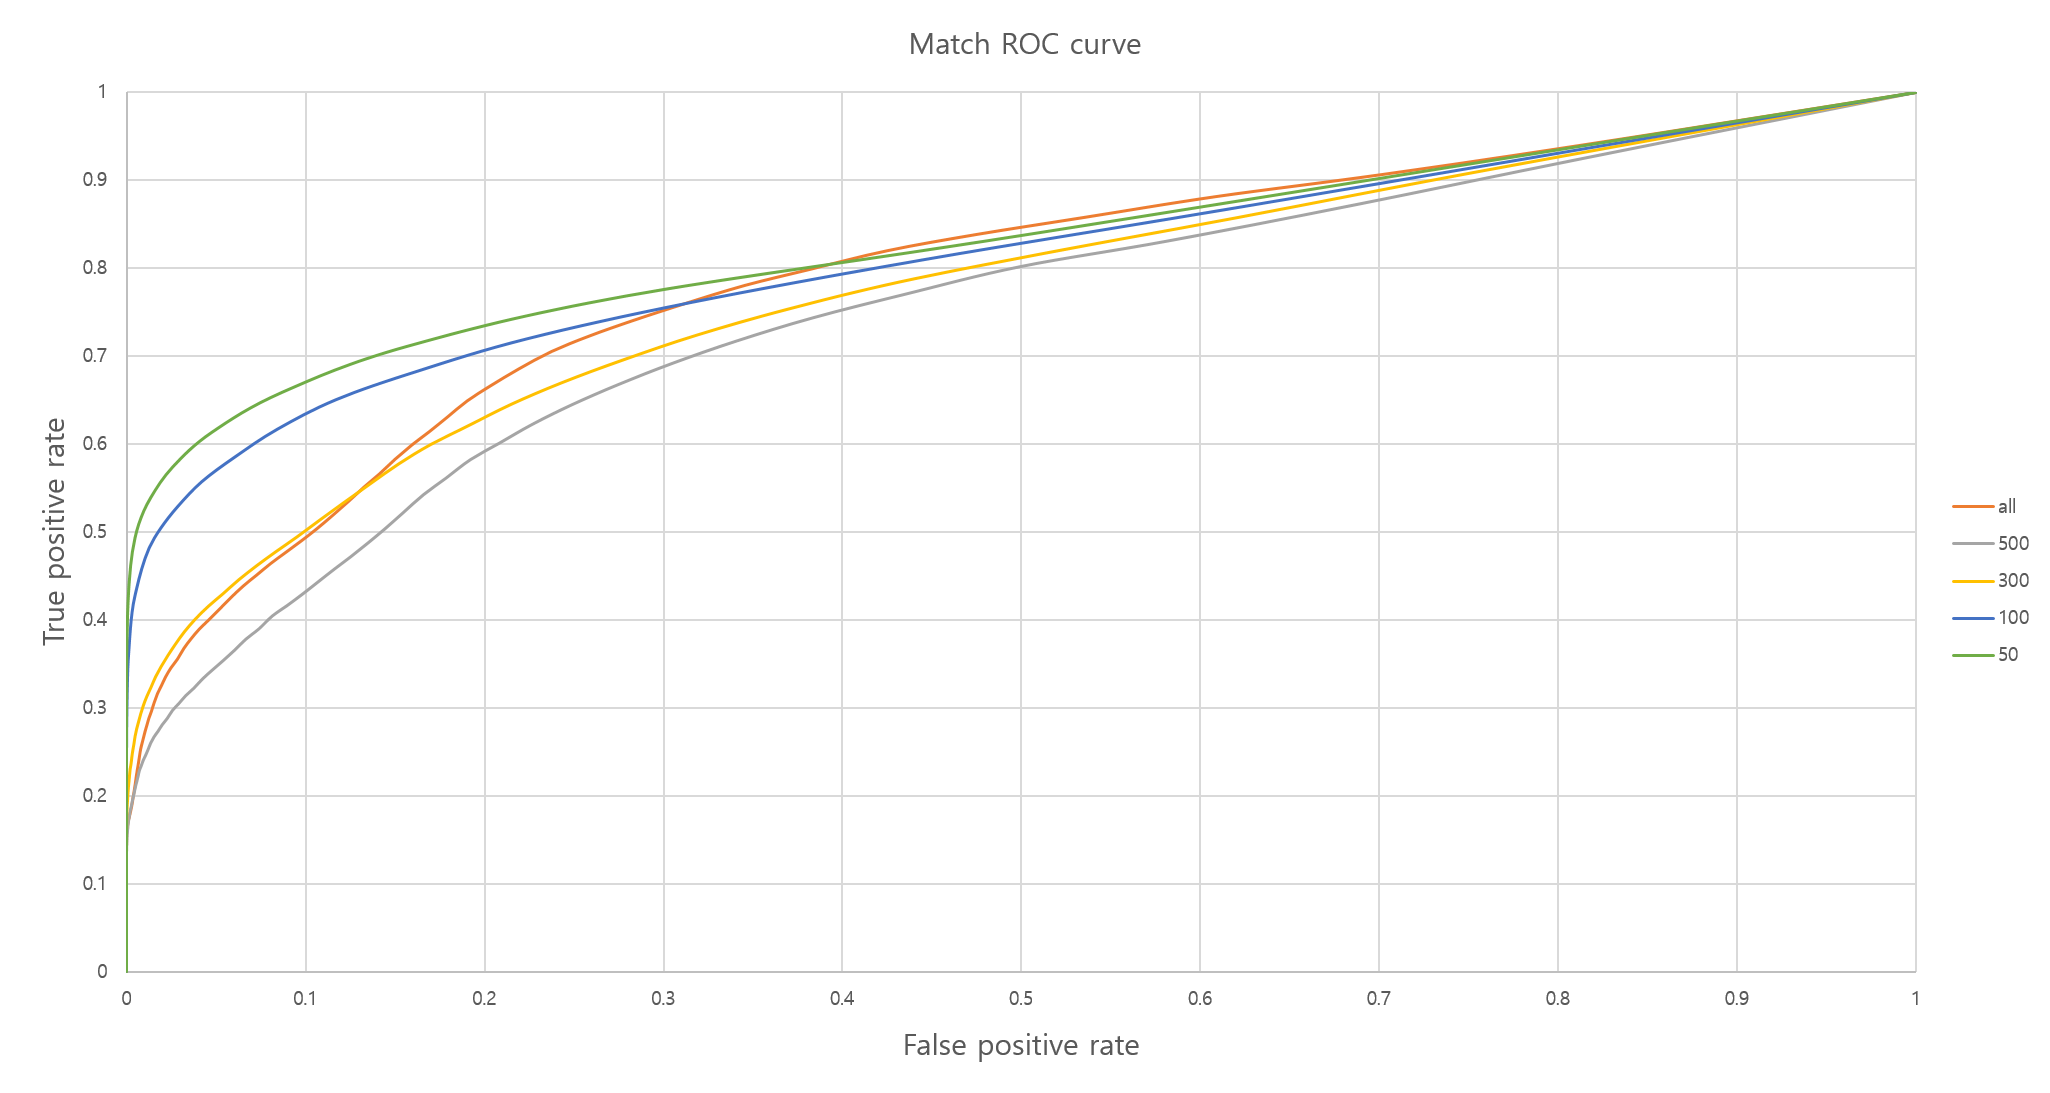
\includegraphics[width=1.0\columnwidth]{4_experiments/roc}
\caption{ROC curve for match rate}
\label{fig:markerless_roc}
\end{figure}

% 이러한 keypoint filtering을 수행하게 되면, miss-match를 유발하는 bad keypoint가 제거되기 때문에 match 결과의 reliability 가 높아진다. 이를 증명하기 위하여 Feature-level에서 Precision\cite{heinly_comparative_2012}을 계산하였다. Precision은 match 결과 구해진 correspondence pair의 수 대비 correct match의 비율로 계산이 된다. 이는 match 결과에 얼마나 miss-match가 적고 correct match의 비율이 높은지를 나타낸다. match 결과 대비 correct match의 비율이 높을수록 이후에 robust pose estimation의 성능에 영향을 미친다.

% When performing keypoint filtering, the bad keypoints causing miss-match are eliminated, which in turn increases the reliability of the match results. To prove this, the precision\cite{heinly_comparative_2012} in the feature-level was calculated. The precision can be calculated as the ratio between the number of the correspondence pairs obtained after matching and the correct matches, indicating the insignificant proportion of mass-match and significant proportion of correction match in the match results. The increase of the ratio between correct match and match results subsequently affects the performance of robust pose estimation. 


% % \begin{figure}[t!]
% % \centering
% % 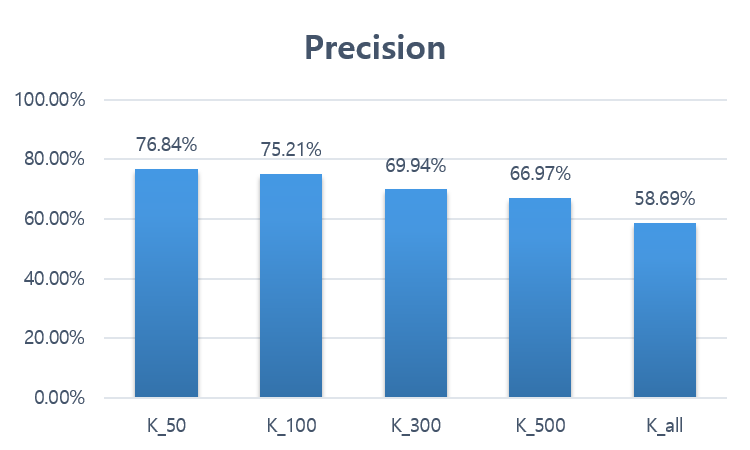
\includegraphics[width=1.0\columnwidth]{4_experiments/precision}
% % \caption{Precision of filtered keypoint database}
% % \label{fig:markerless_precision}
% % \end{figure}

% % \begin{table}[b!]
% % \centering
% % %\resizebox{\columnwidth}{!}{%
% % \begin{tabular}{llllll}
% % \hline
% % \textbf{}                   & \textbf{$K_{50}$} & \textbf{$K_{100}$} & \textbf{$K_{300}$} & \textbf{$K_{500}$} & \textbf{$K_{all}$} \\
% % \textbf{Avg. Match Result}  & 10.098            & 15.618             & 26.747             & 31.409             & 44.859             \\
% % \textbf{Avg. Correct Match} & 7.759             & 11.747             & 18.705             & 21.033             & 26.326             \\
% % \textbf{Precision}          & 76.8\%            & 75.2\%             & 69.9\%             & 67.0\%             & 58.7\%             \\ \hline
% % \end{tabular}
% % %}
% %   \caption{Precision of Filtered Matching}
% %   \label{tab:markerless_precision}
% % \end{table}

% % Precision의 결과는 그림 \ref{fig:markerless_precision}와 표\ref{tab:markerless_precision}에 나타난다. 전체 특징점 집합($K_{all}$)에 비하여 filtered 특징점 집합들이 더 높은 precision을 나타내주었다. 검출되는 특징점의 개수는 줄어들지만, Correct Match의 비율이 높아지기 때문에 높은 Precision을 보여주었다. 이러한 결과는 robst pose estimation의 속도와 성능을 향상시킬 수 있다.

% The results of precision are demonstrated in Table \ref{tab:markerless_precision} and Table \ref{fig:markerless_precision}. The filtered keypoints sets showed higher precision compared to the whole of keypoints set ($K_{all}$). The number of the detected keypoints decreased but the ratio of correct match increased, which showed high precision. Such results are able to improve the speed and performance of robust pose estimation.  
